\documentclass{llncs}
\usepackage[utf8]{inputenc}
\usepackage{verbatim}
\usepackage{multicol}
\usepackage{llncsdoc}
\usepackage{amsmath}
\usepackage{amsfonts}
\usepackage{amssymb}
\usepackage{graphicx}
\usepackage{lmodern}
\usepackage{calc}
\usepackage{enumitem}
\usepackage{algpseudocode}
\usepackage{algorithm}
\usepackage{algorithmicx}

\algsetblockdefx[IfContinue]{IfContinue}{IfContinue}
{0}{0pt}
[0]{}
[1]{\textbf{if} #1 \textbf{continue}}

\algrenewcommand\algorithmicrequire{%
  \makebox[\widthof{\textbf{Output:}}][l]{\textbf{Input:}}}
  
 \algrenewcommand\algorithmicensure{%
  \textbf{Output:}}

\usepackage{color}
\usepackage{gnuplottex}
\usepackage{subcaption}
\usepackage{microtype}
\usepackage[normalem]{ulem}
\captionsetup{compatibility=false}
\usepackage{tikz}
\usetikzlibrary{trees,automata,positioning}
\usepackage{booktabs}
\usepackage{gnuplottex}
\usepackage{xparse}
\usepackage{epstopdf}
% For scaling gnuplottex
\ExplSyntaxOn
\DeclareExpandableDocumentCommand{\convertlen}{ O{cm} m }
 {
  \dim_to_unit:nn { #2 } { 1 #1 } cm
 }
\ExplSyntaxOff

%% For lattice figure
% Set the overall layout of the tree
\tikzstyle{level 1}=[level distance=3.0cm, sibling distance=0.6cm]
\tikzstyle{level 2}=[level distance=3.5cm, sibling distance=0.6cm]
\tikzstyle{level 3}=[level distance=3.5cm, sibling distance=0.6cm]

% Define styles for bags and leafs
\tikzstyle{l1} = [rectangle, text width=5em, text centered]
\tikzstyle{l2} = [rectangle, text width=5em, text centered]
\tikzstyle{l3} = [rectangle, text width=5em, text centered]

% only when using asmthm
%\newtheorem{definition}{Definition}
%\newtheorem{theorem}{Theorem}

\author{Micky Faas \and Matthijs van Leeuwen}
\title{VOUW: Geometric Pattern Mining using the MDL Principle}
\institute{Leiden Institute for Advances Computer Science}
\begin{document}

\section{Experiments and Results}

To asses the practical performance of the VOUW algorithm, we will primarily use the synthetic dataset generator RIL that was developed specifically for this purpose. RIL utilizes random walks to populate a matrix with patterns of a given size and prevalence, up to a specified density. We fill the remainder of the matrix with uniform noise which allows us to think of the density of patterns as the \emph{signal-to-noise ratio} (SNR). The objective of the resulting experiment is that we try to find all of the signal (the patterns) and none of the noise.

\subsection{Metrics for evaluation}

Completely random data (noise) cannot be compressed (citation needed). Therefore if any compression is achieved, structure must be present in the original data. The SNR tells us how much noise is present in the data and thus conveniently gives us an upper bound of how much compression could be achieved. We use the ground truth SNR versus the resulting compression ratio as a benchmark to tell us how close we are in finding all the structure in the ground truth.

Because the compression ratio alone does not tell us the quality of the results, we also compare the ground truth matrix with the compressed result. In order to do this, we use the notion that elements that have been encoded with singleton patterns, could evidently not be compressed. These elements must therefore be noise. We reconstruct the original matrix from the compressed result, while we omit any singleton patterns. This essentially gives us a matrix of `positives' (signal) and `negatives' (noise). By comparing each element with the corresponding element in the ground truth matrix, the `true positives' can be calculated. This subsequently gives us traditional  figures for \emph{precision} and \emph{recall}.

\begin{figure}%
	%\centering%
	\begin{subfigure}[t]{0.5\textwidth}
	%\centering
	\begin{gnuplot}[terminal=epslatex, terminaloptions={color dashed size 6.5cm,6cm font "lmodern,8"}]
		set key box bottom right
		set key width 1.0
		set key height 1.0
		set key spacing 1.1
		set key opaque
		set sample 1000
		set xr [0:.7]
		set yr [0:1]
		set grid xtics lt 0 ls 0
		set grid ytics lt 0 ls 0
		set xlabel 'signal-to-noise ratio'
		set ylabel ''
		plot "data/256_snr_vs_prec_n10.txt" w l lc 1 lw 3 t "precision",\
			 "data/256_snr_vs_recall_n10.txt" w l lc 2 lw 3 t "recall",\
			 "data/256_snr_vs_compr_n10.txt" w l lc 3 lw 3 t "ratio"
	\end{gnuplot}}\
	\caption{The influence of the signal-to-noise ratio in the ground truth on the algorithm's performance}
	\end{subfigure}%
	~
	\begin{subfigure}[t]{0.5\textwidth}
	%\centering
	\begin{gnuplot}[terminal=epslatex, terminaloptions={color dashed size 6.5cm,6cm font "lmodern,8"}]
		set key box bottom right
		set key width 1.0
		set key height 1.0
		set key spacing 1.1
		set key opaque
		set sample 1000
		set xr [0:50]
		set yr [0:1]
		set grid xtics lt 0 ls 0
		set grid ytics lt 0 ls 0
		set xlabel 'Prevalence per pattern'
		set ylabel 'Recall' offset 1,0,0
		plot "data/usage_test_128.txt" using 1:8 w l lc 1 lw 3 t "128",\
			 "data/usage_test_256.txt" using 1:8 w l lc 2 lw 3 t "256",\
			 "data/usage_test_512.txt" using 1:8 w l lc 3 lw 3 t "512",\
			 "data/usage_test_1024.txt" using 1:8 w l lc 4 lw 3 t "1024"
	\end{gnuplot}
	\caption{Prevalence versus quality of the result (recall)}
	\end{subfigure}
\end{figure}

\begin{figure}
\centering
\begin{subfigure}[t]{0.25\textwidth}
\centering

\includegraphics[scale=.9]{img/exp_input_2.png}
\caption{Generated matrix}
\label{fig-example1a}
\end{subfigure}%
~
\begin{subfigure}[t]{0.25\textwidth}
\centering
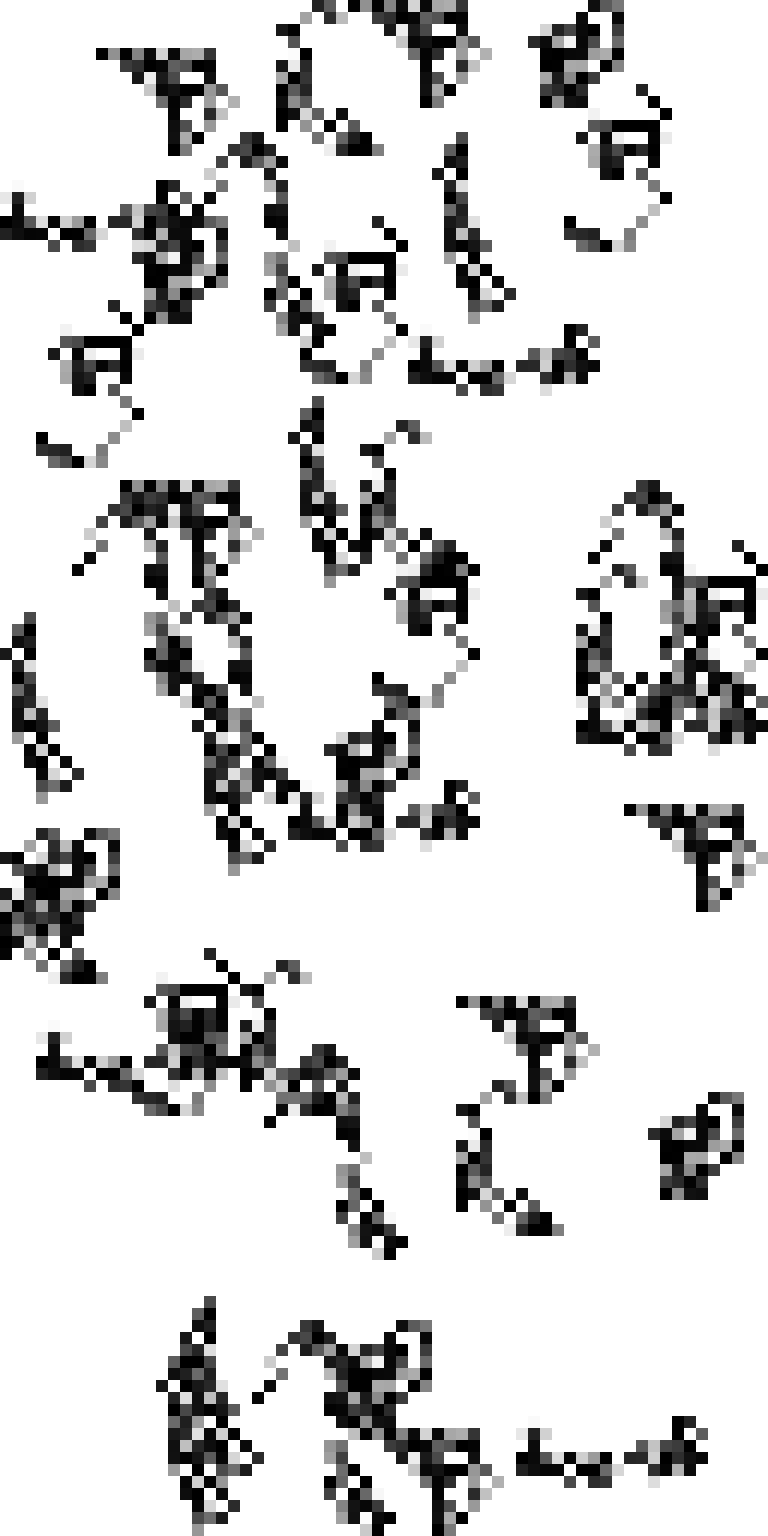
\includegraphics[scale=.9]{img/exp_inputpatterns_2.png}
\caption{Ground truth patterns}
\label{fig-example1b}
\end{subfigure}%
~
\begin{subfigure}[t]{0.25\textwidth}
\centering
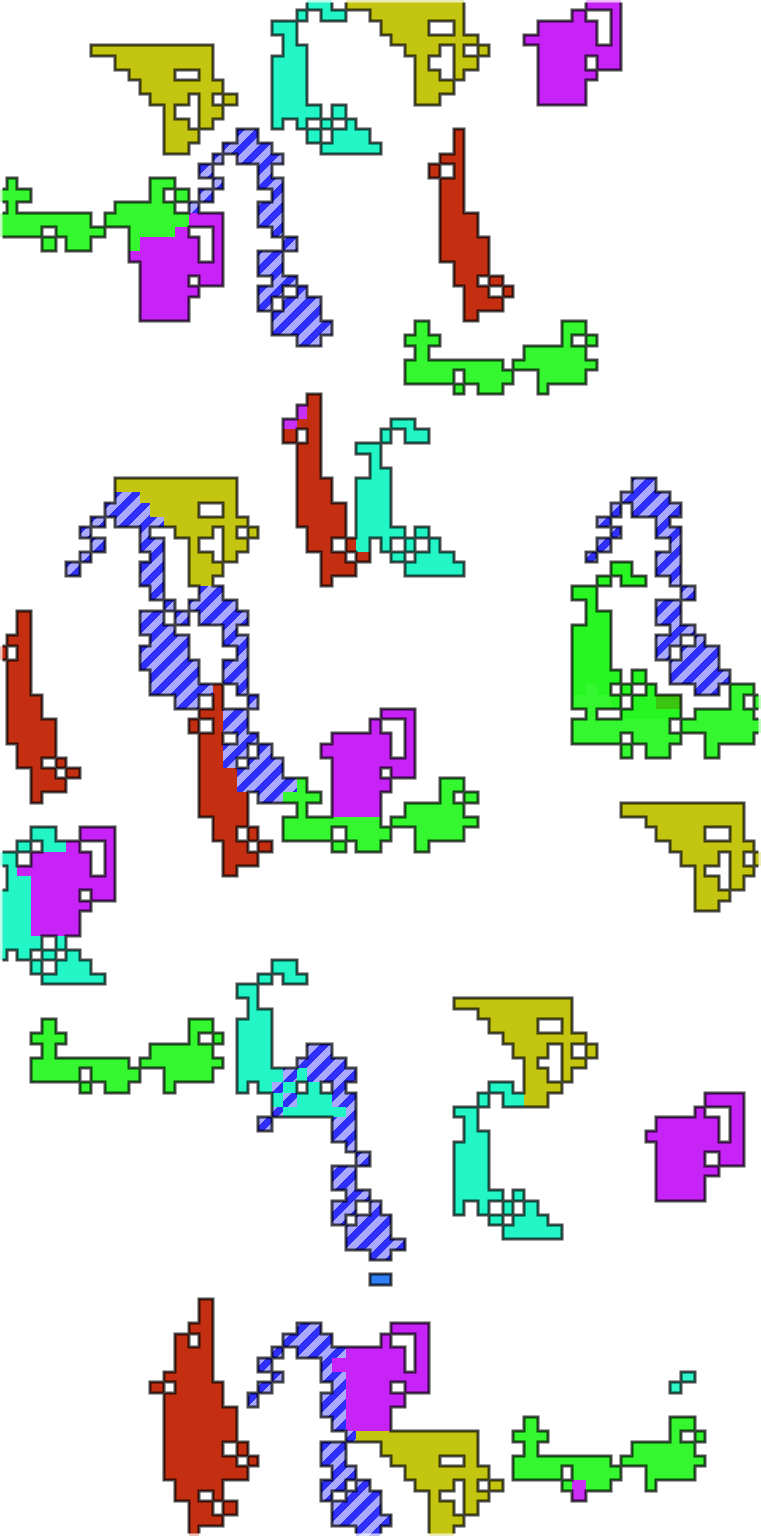
\includegraphics[scale=.9]{img/exp_result_2.png}
\caption{Found patterns}
\label{fig-example1c}
\end{subfigure}%
~
\begin{subfigure}[t]{0.25\textwidth}
\centering

\includegraphics[scale=.9]{img/exp_diff_2.png}
\caption{Difference}
\label{fig-example1c}
\end{subfigure}%
\caption{Example of how synthetic input is generated and evaluated.}

\end{figure}  

\end{document}
